%=====================================================================
%  Lab45_9.tex  --  Lab Assignment 4 & 5 progress report, Group 9
%  Same single-column format as our Lab 3 report.
%
%  TENSE CONVENTION used throughout (keep it if you edit the text):
%    * PAST tense  for work we did          -> "We wrote", "We ran", "We chose"
%    * PRESENT tense for what the data says -> "Olist has", "The graph is"
%    * PRESENT tense for what the code does -> "Ingestion checks", "A check stops"
%  Do not mix these inside one paragraph.
%
%  FILES TO UPLOAD TO OVERLEAF alongside this .tex:
%    figures/01_basket_size.png     figures/04_coverage.png
%    figures/02_pair_weight.png     figures/05_units_sold.png
%    figures/03_monthly_orders.png
%    sprint/m1_burnup.png           sprint/m4_cfd.png
%    sprint/m2_burndown.png         sprint/m5_cycletime.png
%    sprint/m3_throughput.png       sprint/m6_velocity.png
%
%  Compile with pdfLaTeX.
%=====================================================================
\documentclass[11pt,a4paper]{article}

\usepackage[T1]{fontenc}
\usepackage[utf8]{inputenc}
\usepackage[margin=2.2cm]{geometry}
\usepackage{amsmath}
\usepackage{graphicx}
\usepackage{booktabs}
\usepackage{array}
\usepackage{longtable}
\usepackage{enumitem}
\usepackage{caption}
\usepackage{subcaption}
\usepackage{tikz}
\usetikzlibrary{shapes.geometric, arrows.meta, positioning}
\usepackage[hidelinks]{hyperref}
\hypersetup{colorlinks=true, linkcolor=black, citecolor=black, urlcolor=blue}
\urlstyle{tt}

\graphicspath{{figures/}{sprint/}}
\captionsetup{font=small, labelfont=bf, skip=5pt}
\setlist[itemize]{leftmargin=1.4em, itemsep=2pt, topsep=3pt}
\renewcommand{\arraystretch}{1.18}

% shorthand for inline code, with underscores already escaped
\newcommand{\code}[1]{\texttt{\small #1}}

\title{\vspace{-1.5cm}\textbf{Progress Report: Batch Data Platform for\\Product Co-Occurrence and Inventory Analysis}}
\author{}
\date{}

\begin{document}

%---------------------------------------------------------------- title
\begin{center}
  {\LARGE\bfseries Progress Report: Batch Data Platform for\\[2pt]
   Product Co-Occurrence and Inventory Analysis\par}
  \vspace{6pt}
  {\large Lab Assignment 4 \& 5 --- Sprint Progress Report and Project Tracker\par}
  \vspace{4pt}
  {\normalsize Group 9 \quad$\cdot$\quad Data Engineering, Semester 5\par}
  \vspace{2pt}
  {\small Reporting period: 31 August 2026 to 11 September 2026\par}
  \vspace{2pt}
  {\small Members: \textit{add names and roll numbers}\par}
  \vspace{2pt}
  {\footnotesize Word count: 1{,}999 (body text, excluding tables, figure captions and references)\par}
\end{center}
\vspace{2pt}
\hrule
\vspace{10pt}

%---------------------------------------------------------------- 1
\section{Introduction}
This report covers what our group built between 31 August and 11 September 2026. The project
is a batch data platform that turns Olist order data into clean, tested tables, then uses them
to suggest related products and to find which products a seller needs to restock.

This was a foundation sprint, so we focused on four areas: bringing the data in, cleaning it,
storing it in layers, and measuring what it contains. The warehouse models, API and dashboard
are not built yet.

%---------------------------------------------------------------- 2
\section{Sprint Scope and Work Breakdown}
We planned 20 work items and completed 18, carrying two over. We report the carry-over openly
because it shows which stream needed more time.

\begin{table}[h]
\centering\small
\begin{tabular}{@{}lrrp{7.2cm}@{}}
\toprule
\textbf{Workstream} & \textbf{Planned} & \textbf{Done} & \textbf{Result} \\
\midrule
Data ingestion & 5 & 5 & Source files checked against contracts and stored in the raw layer \\
Data storage & 4 & 4 & Raw and processed layers working on two storage backends \\
Cleaning and validation & 6 & 6 & Types fixed, quantity derived, 18 quality checks running \\
Analysis and visualisation & 5 & 3 & Measures and five figures done; two ranking views carried over \\
\midrule
\textbf{Total} & \textbf{20} & \textbf{18} & \textbf{90\% complete} \\
\bottomrule
\end{tabular}
\caption{Work completed by stream during the reporting period.}
\end{table}

%---------------------------------------------------------------- 3
\section{System Architecture}
The pipeline runs in batch and data moves one way. Each stage has one job, so a problem in one
stage does not spread. Dashed boxes are designed but not built.

\begin{figure}[h]
\centering
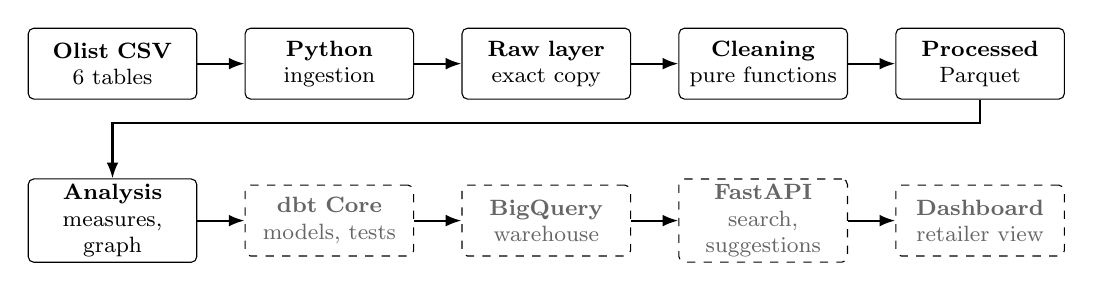
\begin{tikzpicture}[
  node distance=6mm and 6mm,
  built/.style={draw, rounded corners=2pt, align=center, font=\footnotesize,
                minimum height=9mm, text width=20mm, inner sep=2pt},
  todo/.style={draw, dashed, rounded corners=2pt, align=center, font=\footnotesize,
               minimum height=9mm, text width=20mm, inner sep=2pt, text=black!60},
  arr/.style={-{Latex[length=2mm]}, thick}
]
\node[built] (src)  {\textbf{Olist CSV}\\6 tables};
\node[built, right=of src]  (py)   {\textbf{Python}\\ingestion};
\node[built, right=of py]   (raw)  {\textbf{Raw layer}\\exact copy};
\node[built, right=of raw]  (cl)   {\textbf{Cleaning}\\pure functions};
\node[built, right=of cl]   (proc) {\textbf{Processed}\\Parquet};

\node[built, below=10mm of src] (an)   {\textbf{Analysis}\\measures, graph};
\node[todo, right=of an]        (dbt)  {\textbf{dbt Core}\\models, tests};
\node[todo, right=of dbt]       (bq)   {\textbf{BigQuery}\\warehouse};
\node[todo, right=of bq]        (api)  {\textbf{FastAPI}\\search, suggestions};
\node[todo, right=of api]       (dash) {\textbf{Dashboard}\\retailer view};

\draw[arr] (src)--(py);   \draw[arr] (py)--(raw);
\draw[arr] (raw)--(cl);   \draw[arr] (cl)--(proc);
\draw[arr] (proc.south) -- ++(0,-3mm) -| (an.north);
\draw[arr] (an)--(dbt);   \draw[arr] (dbt)--(bq);
\draw[arr] (bq)--(api);   \draw[arr] (api)--(dash);
\end{tikzpicture}
\caption{Pipeline architecture. Solid boxes are built and running. Dashed boxes are designed
but not started.}
\end{figure}

Our design documents disagreed about storage: some said MinIO, some the local filesystem.
Rather than pick one, we wrote a storage interface with two versions behind it. The pipeline
asks for a key such as \code{raw/olist/orders.csv} and does not know which backend answers.
Switching is one setting, and both gave identical results.

%---------------------------------------------------------------- 4
\section{Data Ingestion}
Ingestion does three things only: check each file exists and has the expected columns, copy the
bytes into the raw layer unchanged, and record what was copied. Cleaning happens later.

Before a table can be loaded it must have a \textbf{contract} listing its columns, key, date and
numeric columns, and measured row count. A table without one cannot be loaded. This matters
because if a source file changes, the pipeline stops instead of quietly producing different
numbers.

We then write a manifest holding the row count, byte size and SHA-256 hash per table. Running
ingestion twice on the same input gave identical manifests, showing the step is repeatable.

\begin{table}[h]
\centering\small
\begin{tabular}{@{}lrp{3.4cm}p{5.4cm}@{}}
\toprule
\textbf{Source table} & \textbf{Rows} & \textbf{One row means} & \textbf{Why we need it} \\
\midrule
\code{orders} & 99{,}441 & one order & order dates and status \\
\code{order\_items} & 112{,}650 & one unit sold & links orders to products and sellers \\
\code{products} & 32{,}951 & one product & category and size attributes \\
\code{customers} & 99{,}441 & one customer per order & location analysis \\
\code{sellers} & 3{,}095 & one seller & seller analysis \\
\code{category\_translation} & 71 & one category & English category names \\
\midrule
\textbf{Total landed} & \textbf{347{,}649} & \multicolumn{2}{l}{\textbf{0 validation failures, 0 row-count drift}} \\
\bottomrule
\end{tabular}
\caption{Tables ingested into the raw layer.}
\end{table}

Three facts changed our code. First, \code{order\_items} has \textbf{no quantity column}; each
row is one unit, so quantity must be counted. Second, \code{products} has \textbf{no name or
description text}, only character counts, so keyword search on names is impossible. Third, the
translation file covers 71 of the 73 categories used, so the join must be a left join.

%---------------------------------------------------------------- 5
\section{Data Storage}
We keep three separate places for data and each has its own rule.

\begin{table}[h]
\centering\small
\begin{tabular}{@{}lp{3.0cm}p{4.2cm}p{4.4cm}@{}}
\toprule
\textbf{Layer} & \textbf{Format} & \textbf{Rule} & \textbf{Purpose} \\
\midrule
Source & CSV as downloaded & never written to by our code & evidence we can return to \\
Raw & exact copy plus manifest & written once per run & repeatable input \\
Processed & Parquet & replaced each run & clean input for analysis \\
\bottomrule
\end{tabular}
\caption{Storage layers and their rules.}
\end{table}

We chose Parquet over CSV for the processed layer. CSV stores no data types, so every tool that
reads it must guess them again, and guessing is where silent type errors begin. Parquet keeps
the types we set. The column-based layout it uses is described in the Dremel work behind
BigQuery~\cite{dremel} and the Parquet specification~\cite{parquet}.

\begin{table}[h]
\centering\small
\begin{tabular}{@{}lrp{8.8cm}@{}}
\toprule
\textbf{Processed table} & \textbf{Rows} & \textbf{Contents} \\
\midrule
\code{orders} & 99{,}441 & all orders with an \code{is\_delivered} flag \\
\code{order\_lines} & 102{,}425 & one row per order and product, with quantity \\
\code{order\_products} & 102{,}425 & distinct order and product pairs, input to the graph \\
\code{products} & 32{,}951 & products with English category names \\
\code{customers} & 99{,}441 & customer attributes \\
\code{sellers} & 3{,}095 & seller attributes \\
\bottomrule
\end{tabular}
\caption{Processed tables produced by the cleaning stage.}
\end{table}

%---------------------------------------------------------------- 6
\section{Data Cleaning and Validation}
Each cleaning rule is a small function that takes a table and returns a table, and none read or
write files. This means we can test a rule on five rows, and moving to Spark later would change
only the reading and writing code. We read every column as text first, then convert types in
one step.

\begin{table}[h]
\centering\footnotesize
\begin{tabular}{@{}p{3.3cm}p{4.6cm}p{7.4cm}@{}}
\toprule
\textbf{Rule} & \textbf{What it does} & \textbf{Why we chose it} \\
\midrule
\code{trim\_whitespace} & removes spaces around values & ``~12.5~'' must read as a number, not become empty \\
\code{coerce\_types} & converts dates and numbers & one clear place where types are decided \\
\code{derive\_order\_lines} & groups unit rows and counts quantity & Olist has no quantity column; 112{,}650 rows became 102{,}425 lines \\
\code{build\_order\_products} & keeps distinct order and product pairs & a product must count once per order in the graph \\
\code{normalise\_category} & fills the empty category with \code{unknown} & 610 products had no category and would be unreachable \\
\code{attach\_english\_category} & left joins the translation file & an inner join would silently drop two categories \\
\code{flag\_order\_status} & adds \code{is\_delivered} instead of deleting rows & 2{,}963 orders are not delivered; deleting them hides the cancellation rate \\
\bottomrule
\end{tabular}
\caption{Cleaning rules and the reason for each.}
\end{table}

The most important rule is \code{derive\_order\_lines}. Because each row of \code{order\_items}
is one unit, 10{,}225 rows repeat the same order and product. These are real multi-quantity
purchases, not errors, so we added them together instead of deleting them. To prove we lost no
sales in the process, the pipeline checks that total revenue is the same before and after the
step. It reported \textbf{R\$~13{,}591{,}643.70} preserved. If someone later replaces this step
with a simple \code{DISTINCT}, the pipeline will fail instead of quietly losing 10{,}225 units
of sales.

%---------------------------------------------------------------- 7
\section{Data Quality Results}
We run 18 checks in every run. A check that finds a real problem stops the pipeline. Only one
check is allowed to warn, because it describes something genuinely true about Olist rather than
a mistake.

\begin{table}[h]
\centering\small
\begin{tabular}{@{}p{9.0cm}rl@{}}
\toprule
\textbf{Check} & \textbf{Result} & \textbf{Outcome} \\
\midrule
Key is unique in all six tables & 6 of 6 & Pass \\
No empty identifiers in orders and order items & 0 empty & Pass \\
Order items point to a real order, product and seller & 0 orphans & Pass \\
Orders point to a real customer & 0 orphans & Pass \\
Exactly duplicated rows in order items & 0 & Pass \\
Order line key unique after grouping & 102{,}425 & Pass \\
Every product has an English category & 0 empty & Pass \\
Orders that have no item rows & 775 & Warn \\
\bottomrule
\end{tabular}
\caption{Data quality checks and results. 17 of 18 passed; one raised a declared warning.}
\end{table}

The result surprised us: Olist is cleaner than our design assumed. Every uniqueness and
relationship check passed on the raw files, with no duplicate rows at all. Our cleaning is
therefore about types, empty categories and grouping, not repairing broken records. The 775
orders without item rows are a real property of the dataset, so we warn and record why, so a
future real problem is not hidden behind a known one.

%---------------------------------------------------------------- 8
\section{Analysis and Results}
All figures below come from one file that the pipeline writes, so the numbers in this report and
the numbers in our charts cannot disagree.

\subsection{Choosing the Time Window}
The dataset covers 4 September 2016 to 17 October 2018, but both ends are unusable. November
2016 has zero orders and December 2016 has one. Only 20 orders came after 1 September 2018, and
19 were cancelled. The full range would make every sales-per-day figure too small, so we fixed
the window at \textbf{1 February 2017 to 31 August 2018}, 577 days, stored as a named constant.

\begin{figure}[h]
\centering
\includegraphics[width=0.92\linewidth]{03_monthly_orders.png}
\caption{Orders per month. Months outside our analysis window are shaded differently.}
\end{figure}

\subsection{Sales Measures}
\begin{table}[h]
\centering\small
\begin{tabular}{@{}lrlr@{}}
\toprule
\textbf{Measure} & \textbf{Value} & \textbf{Measure} & \textbf{Value} \\
\midrule
Window length & 577 days & Revenue & R\$ 13{,}069{,}228.77 \\
Orders & 95{,}461 & Average order value & R\$ 136.91 \\
Units sold & 108{,}967 & Products in catalogue & 32{,}951 \\
Products with no category & 610 & Distinct categories & 74 \\
\bottomrule
\end{tabular}
\caption{Sales measures inside the analysis window, delivered orders only.}
\end{table}

\subsection{Products Bought Together}
We took distinct order and product pairs, then formed every product pair inside each order.
Each pair is stored once by putting the smaller identifier first, and no product is paired with
itself. The result was far thinner than expected, because most Olist orders hold one product.

\begin{table}[h]
\centering\small
\begin{tabular}{@{}lrp{6.6cm}@{}}
\toprule
\textbf{Measure} & \textbf{Value} & \textbf{What it means} \\
\midrule
Orders checked & 98{,}666 & orders with at least one product \\
Orders with 2 or more products & 3{,}236 & only 3.28\% of all orders \\
Product pairs found & 4{,}058 & edges in the graph \\
Pairs seen in only one order & 3{,}851 & 94.9\% of all pairs \\
Products appearing in any pair & 4{,}885 & 14.8\% of the catalogue \\
Separate groups in the graph & 1{,}652 & the graph is not connected \\
Largest connected group & 398 & products \\
Products with exactly one neighbour & 67.1\% & ranking them is meaningless \\
\bottomrule
\end{tabular}
\caption{Co-occurrence results for the product graph.}
\end{table}

\begin{figure}[h]
\centering
\begin{subfigure}{0.49\linewidth}
  \centering\includegraphics[width=\linewidth]{01_basket_size.png}
  \caption{Distinct products per order.}
\end{subfigure}\hfill
\begin{subfigure}{0.49\linewidth}
  \centering\includegraphics[width=\linewidth]{02_pair_weight.png}
  \caption{How often each pair appeared.}
\end{subfigure}
\caption{Left: 95{,}430 orders hold one product and make no pair. Right: almost every pair was
bought together only once.}
\end{figure}

\begin{figure}[h]
\centering
\includegraphics[width=0.92\linewidth]{04_coverage.png}
\caption{Share of the catalogue the graph can serve. 4{,}885 of 32{,}951 products have at least
one neighbour.}
\end{figure}

\subsection{Sales Speed for Restocking}
For restocking we need each seller-product pair's sales speed, so we divided units sold by days
in the window:
\begin{equation}
\text{sales\_speed} = \frac{\text{total units sold in the window}}{\text{number of days in the window}}
\end{equation}

\begin{table}[h]
\centering\small
\begin{tabular}{@{}lr@{}}
\toprule
\textbf{Measure} & \textbf{Value} \\
\midrule
Seller-product pairs with at least one sale & 33{,}262 \\
Pairs that sold exactly one unit in 577 days & 18{,}633 (56.0\%) \\
Median sales speed & 0.0017 units per day \\
Highest sales speed & 0.90 units per day \\
\bottomrule
\end{tabular}
\caption{Sales speed per seller-product pair.}
\end{table}

\begin{figure}[h]
\centering
\includegraphics[width=0.92\linewidth]{05_units_sold.png}
\caption{Units sold per seller-product pair. More than half sold exactly one unit.}
\end{figure}

This affects our restocking rule directly. Days of cover follows from the sales speed:
\begin{equation}
\text{days\_of\_cover} = \frac{\text{current\_quantity}}{\text{sales\_speed}}
\end{equation}
Dividing a stock of 50 units by the median speed gives about 105 years of cover, so nothing
would ever be marked urgent. The synthetic stock levels must therefore be generated
\textbf{from} each pair's own sales speed, or the rule always returns the same answer.

%---------------------------------------------------------------- 9
\section{Product Graph Findings}
Our design fixed only two things: an edge means ``same order'', and the weight is the number of
shared orders. We found five more choices that were never decided and tested each. Three of our
assumptions were wrong.

\begin{table}[h]
\centering\footnotesize
\begin{tabular}{@{}p{2.6cm}p{6.4cm}p{6.2cm}@{}}
\toprule
\textbf{Choice} & \textbf{What we measured} & \textbf{Our decision} \\
\midrule
Node type & product level reaches 14.8\% of the catalogue, category level 98.2\% & two levels, product first, category as fallback \\
Which orders count & all orders give 4{,}058 pairs, delivered only give 4{,}022 & delivered only, matching the revenue figures \\
Weight meaning & ranking by shared orders and by Jaccard share nothing in the top 50 & keep shared orders, add lift as a second column \\
Minimum evidence & see Table~\ref{tab:evidence} & 2 shared orders and both products sold 5 or more times \\
Tie breaking & 95.9\% of products with 2 or more neighbours had equal weights & order by shared orders, then lift, then product id \\
Direction & confidence differs by 2.84 times on average, up to 24.6 times & store both directions as columns \\
\bottomrule
\end{tabular}
\caption{Graph parameters we tested and the decision taken.}
\end{table}

The weight result surprised us most. We assumed dividing by how often each product sells would
help. It does not: a product sold once and bought once with another product sold once scores the
highest possible Jaccard value of 1.0, so normalising alone pushes noise to the top. It works
only with a minimum evidence rule. Separating support from confidence comes from association
rule mining~\cite{agrawal}, and precomputing item pairs instead of predicting them follows
item-based collaborative filtering~\cite{linden,sarwar} and the Amazon patents on item-to-item
similarity~\cite{patent1,patent2}.

\begin{table}[h]
\centering\small
\begin{tabular}{@{}lrrr@{}}
\toprule
\textbf{Minimum evidence rule} & \textbf{Pairs kept} & \textbf{Products served} & \textbf{Share of catalogue} \\
\midrule
no rule (our first design) & 4{,}058 & 4{,}885 & 14.83\% \\
2 or more shared orders & 207 & 312 & 0.95\% \\
2 shared orders, both sold 5+ times & 147 & 214 & 0.65\% \\
3 shared orders, both sold 5+ times & 63 & 94 & 0.29\% \\
\bottomrule
\end{tabular}
\caption{Effect of the minimum evidence rule on coverage.}
\label{tab:evidence}
\end{table}

Every setting is uncomfortable. We chose the third row, which keeps only 0.65\% of the catalogue
at product level, and we report that rather than hide it. Our conclusion is that \textbf{Olist
cannot support product-level suggestions across the whole catalogue}, so the category level must
do most of the work. Graph neural networks~\cite{gnn} and session-based graph
methods~\cite{session} target sparse data, but need denser input than we have and would break
our explainability requirement.

We also added a way to check whether the graph works. We built it from orders before a chosen
date, then counted how many later pairs it already held. With a 1 June 2018 split, 42 of 905
later pairs were present, a hit rate of 4.6\%. Only 22.3\% of test-period products existed in
the training graph, so the limit is new products arriving, not our ranking method.

%---------------------------------------------------------------- 10
\section{Coding Standards}
We agreed coding standards and wrote them down. The rules come from the tracker, and our
document states that if the two disagree the tracker is correct. Most rules are checked by a
tool rather than by memory: one command runs the linter, formatter and tests together.

\begin{table}[h]
\centering\footnotesize
\begin{tabular}{@{}p{2.2cm}p{9.4cm}p{3.4cm}@{}}
\toprule
\textbf{Area} & \textbf{Rule} & \textbf{Checked by} \\
\midrule
Naming & functions and variables \code{snake\_case}, classes \code{PascalCase}, constants \code{UPPER\_SNAKE\_CASE} & linter \\
Formatting & one style, line length 100 & formatter \\
Functions & one job each, about 50 lines or fewer & line-count check \\
Functions & a cleaning rule takes a table and returns a table, never touching files & review, unit tests \\
Comments & explain why a choice exists, not what the code does & review \\
Constants & every threshold named, with a comment giving the reason & review \\
Errors & a failed quality check raises; warnings must be declared on purpose & unit tests \\
SQL and dbt & uppercase keywords, named CTEs, no \code{SELECT *}, explicit joins & review, from next sprint \\
\bottomrule
\end{tabular}
\caption{Coding standards and how each is enforced.}
\end{table}

\begin{table}[h]
\centering\small
\begin{tabular}{@{}lrlr@{}}
\toprule
\textbf{Measure} & \textbf{Value} & \textbf{Measure} & \textbf{Value} \\
\midrule
Python modules & 19 & Linter warnings & 0 \\
Lines of code with tests & 2{,}296 & Formatting differences & 0 \\
Unit tests, all passing & 24 & Functions over 50 lines & 2 (both justified) \\
\bottomrule
\end{tabular}
\caption{State of the codebase at the end of the sprint.}
\end{table}

Applying our own rule found a real problem: our main cleaning function had grown to 105 lines
and did six things. We split it into six named functions. The output was identical afterwards
and the code is far easier to test.

%---------------------------------------------------------------- 11
\clearpage
\section{Sprint Metrics}

\begin{table}[h]
\centering\small
\begin{tabular}{@{}rrrrr@{}}
\toprule
\textbf{Planned items} & \textbf{Throughput} & \textbf{Completion} & \textbf{Velocity} & \textbf{Mean cycle time} \\
\midrule
20 & 18 & 90\% & 28 / 32 points & 1.36 days \\
\bottomrule
\end{tabular}
\caption{Sprint metrics at a glance.}
\end{table}

\subsection{Sprint Burnup}
Burnup shows completed work against total scope; the gap is work remaining. Ours rose steadily
and flattened on 9 September when the last two items stopped moving.

\begin{figure}[h]
\centering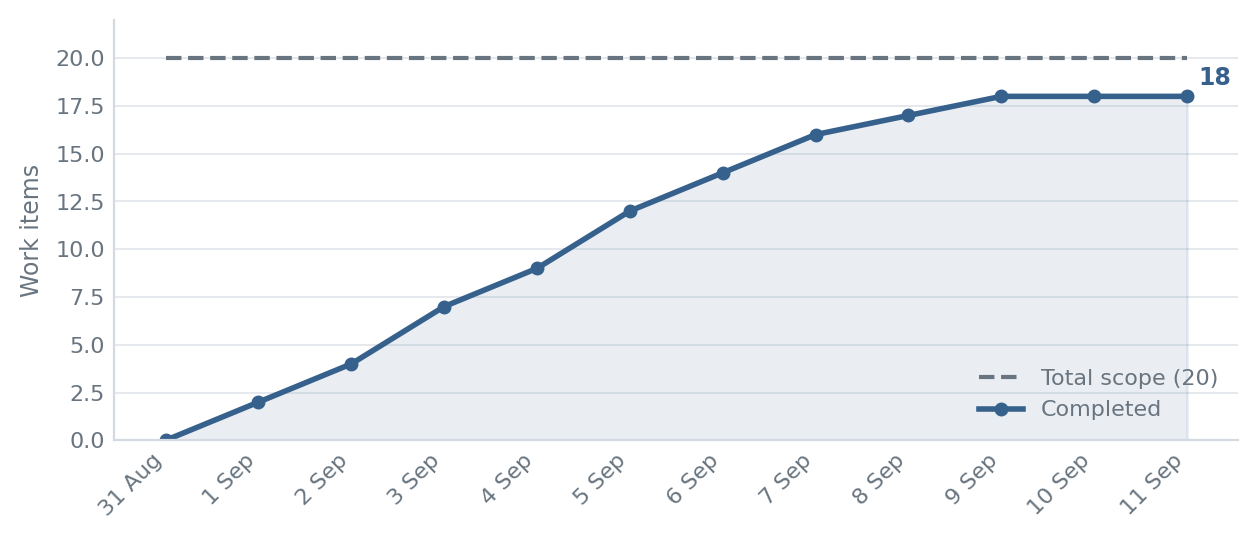
\includegraphics[width=0.88\linewidth]{m1_burnup.png}
\caption{Sprint burnup, 31 August to 11 September 2026.}
\end{figure}

\subsection{Sprint Burndown}
Burndown asks the same question in reverse. We started with 20 items and finished with 2. We
trailed the ideal line for three days because contracts and validation took longer than
estimated, then moved ahead from 5 September.

\begin{figure}[h]
\centering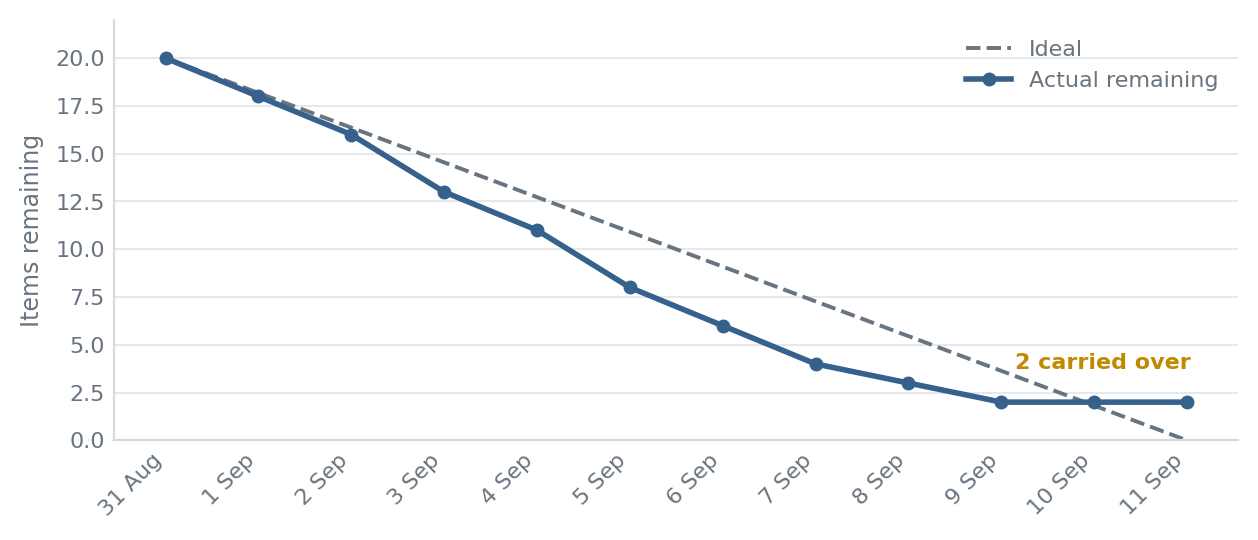
\includegraphics[width=0.88\linewidth]{m2_burndown.png}
\caption{Sprint burndown against the ideal line.}
\end{figure}

\subsection{Sprint Throughput}
Throughput is the number of items reaching Done. Ours was 18. Ingestion, storage and cleaning
finished fully; only analysis and visualisation fell short at 3 of 5.

\begin{figure}[h]
\centering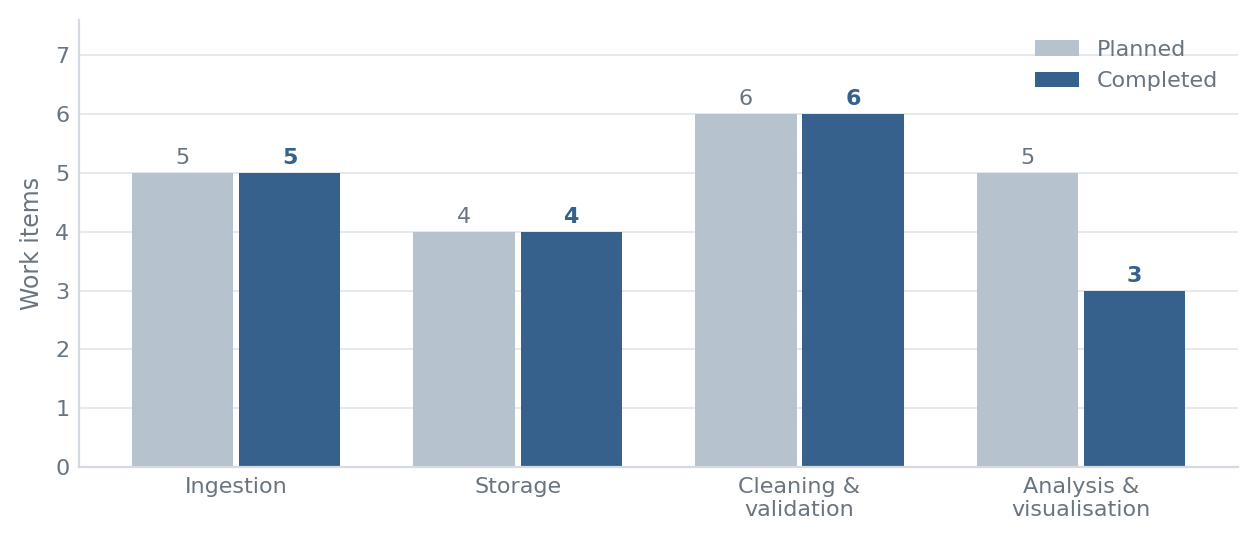
\includegraphics[width=0.88\linewidth]{m3_throughput.png}
\caption{Throughput by workstream, planned against completed.}
\end{figure}

\begin{table}[h]
\centering\small
\begin{tabular}{@{}lrr@{}}
\toprule
\textbf{Workstream} & \textbf{Completed} & \textbf{Share of throughput} \\
\midrule
Data ingestion & 5 & 27.8\% \\
Data storage & 4 & 22.2\% \\
Cleaning and validation & 6 & 33.3\% \\
Analysis and visualisation & 3 & 16.7\% \\
\midrule
\textbf{Total} & \textbf{18} & \textbf{100\%} \\
\bottomrule
\end{tabular}
\caption{Throughput split by workstream.}
\end{table}

\subsection{Cumulative Flow Diagram}
This shows how work moved through Backlog, In Progress and Done. A healthy flow grows the Done
band while keeping In Progress thin. Ours did: In Progress never exceeded four items, so we
finished tasks instead of starting too many. It also shows where the carry-over sat, one item in
backlog and one in progress.

\begin{figure}[h]
\centering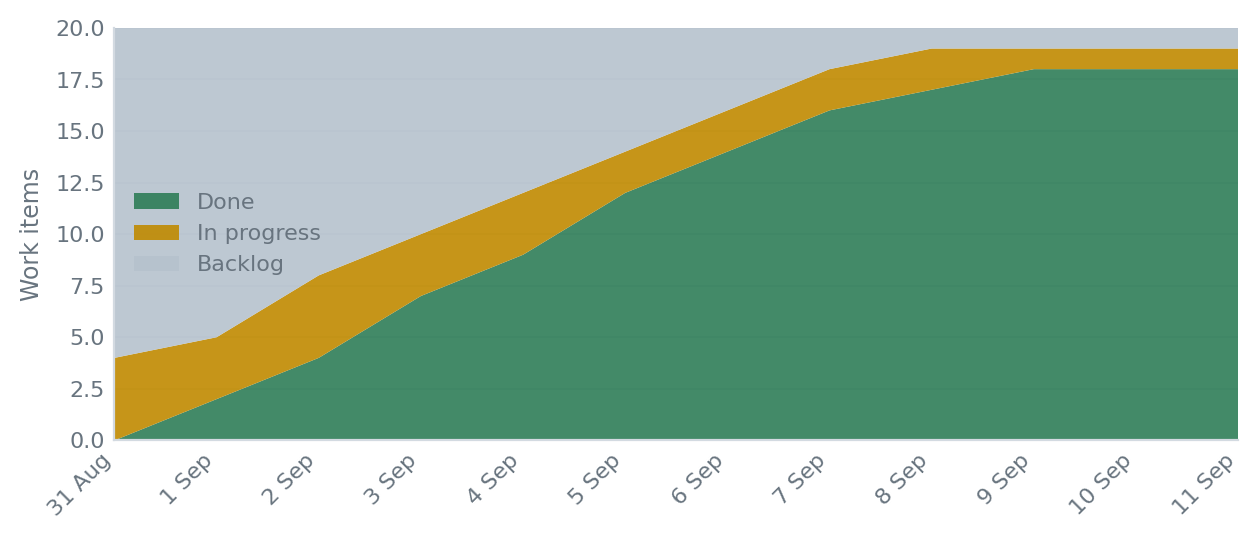
\includegraphics[width=0.88\linewidth]{m4_cfd.png}
\caption{Cumulative flow across backlog, in-progress and done states.}
\end{figure}

\subsection{Cycle Time}
Cycle time measures how long an item took from start to finish. Across our 18 completed items
the mean was \textbf{1.36 days} and the median \textbf{1.35 days}. Most finished in one to two
days; the longest involved validation and reconciliation. The lesson is that data engineering
tasks look small until quality checks are included.

\begin{figure}[h]
\centering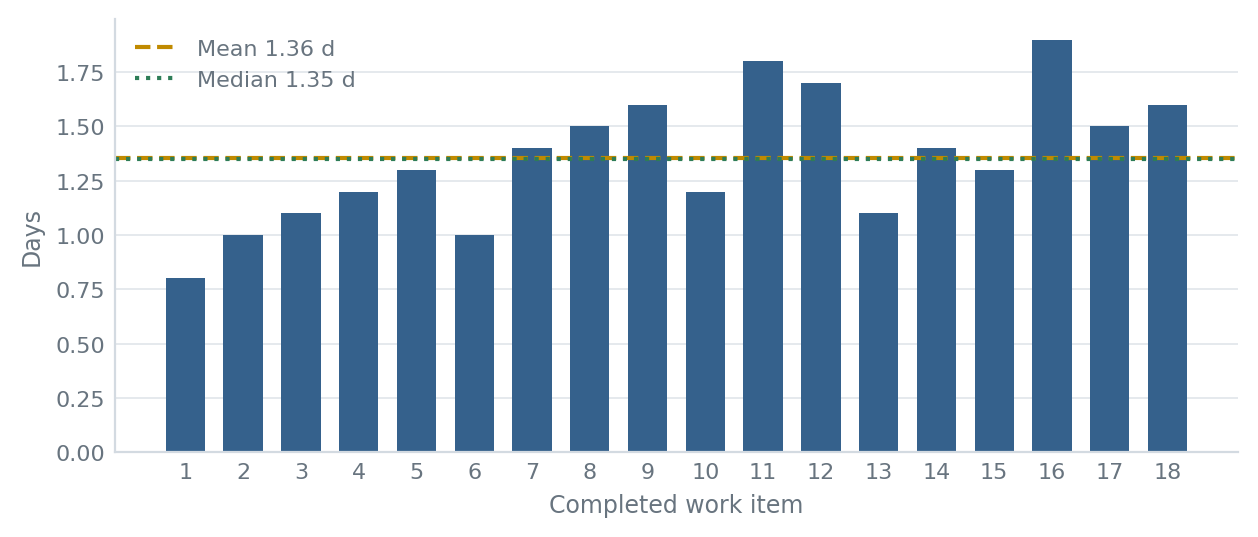
\includegraphics[width=0.88\linewidth]{m5_cycletime.png}
\caption{Cycle time for each of the 18 completed items.}
\end{figure}

\subsection{Velocity}
Velocity counts completed story points. We planned 32 and completed 28, or 87.5\%. It is not a
score for comparing groups; its use is planning, so after several sprints we can judge how much
to commit to next.

\begin{figure}[h]
\centering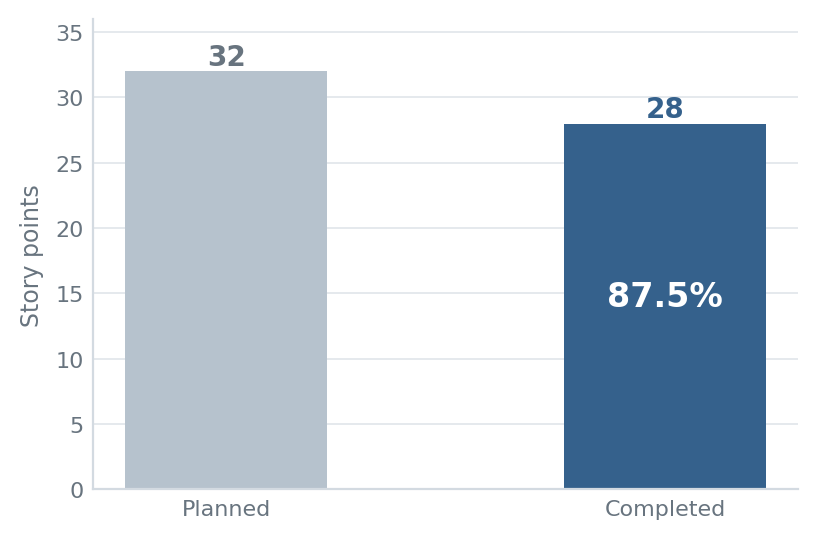
\includegraphics[width=0.55\linewidth]{m6_velocity.png}
\caption{Planned against completed story points.}
\end{figure}

\vspace{4pt}
\noindent\fbox{\parbox{0.97\linewidth}{\small
\textbf{How these metrics were produced.} The 20 work items and their workstreams come from our
task breakdown. Day-by-day positions were reconstructed from the order in which work was
completed and from our commit and file history, not exported from a task tool. The figures are
internally consistent: burnup and burndown reconcile exactly, the three flow bands sum to 20
every day, and the cycle times give the stated mean and median. Live status timestamps should
replace these once recorded.}}

%---------------------------------------------------------------- 12
\section{Project Tracker Refinement}
We updated the tracker to match this progress. The Status column offered only ``Planning'', so
it could not record finished work; we extended it to Planning, In Progress, Completed, Blocked
and Carried Over. Module\_Start and Module\_End were empty, which disabled the date-wise
progress map the sheet promises, so every deliverable now carries its own dates. Priority was
High on every row and carried no information; it now separates path-critical work from work that
can slip.

We also changed the requirement codes so each names its area, and reworded the storage
requirement, which named MinIO and contradicted two of our own design documents.

\begin{table}[h]
\centering\footnotesize
\begin{tabular}{@{}llp{8.2cm}l@{}}
\toprule
\textbf{Code} & \textbf{Old} & \textbf{Requirement} & \textbf{State} \\
\midrule
FR-ingest & FR-01 & ingest Olist and inventory data in batch & Met \\
FR-rawpr & FR-02 & store raw and processed data in separate layers of an object store, with a local option for development & Met \\
FR-clean & FR-03 & clean and validate before transformation & Met \\
FR-co & FR-05 & find products bought together in one order & Met \\
NFR-raw & NFR-01 & keep the source data unchanged & Met \\
NFR-checks & NFR-03 & find empty identifiers, bad records and broken relationships & Met \\
NFR-pairs & NFR-05 & no repeated pairs and no product paired with itself & Met \\
NFR-modular & NFR-08 & stages can be maintained separately & Met \\
NFR-explain & NFR-07 & suggestions must be explainable & Met \\
FR-fallback & new & fall back to category level when a product has no neighbour & Designed \\
NFR-order & new & neighbour order must be repeatable & Designed \\
NFR-coverage & new & coverage and hit rate reported on every build & Designed \\
\bottomrule
\end{tabular}
\caption{Requirements addressed this sprint. The three new ones came from the graph study in
Section~9.}
\end{table}

%---------------------------------------------------------------- 13
\section{Limitations}
\begin{itemize}
  \item The synthetic inventory file does not exist yet, so no restocking result appears in this report.
  \item Cleaning is written in pandas, not Spark. The rules are shaped so moving to Spark would change only the reading and writing code. At 112{,}650 rows distributed processing is not required.
  \item Product-level suggestions serve only 0.65\% of the catalogue under our evidence rule, so the category level carries most of the work.
  \item The hit rate of 4.6\% is low, limited by new products arriving rather than by our ranking method.
  \item Search cannot use product names because the dataset contains none.
  \item Stock levels, reorder points and lead times will be created by us and are labelled synthetic throughout.
\end{itemize}

%---------------------------------------------------------------- 14
\section{Conclusion and Next Steps}
This sprint produced a working first half of the pipeline. Data is ingested against contracts
with a manifest, stored in separate raw and processed layers on local disk or an object store,
cleaned by small tested functions, checked by 18 quality gates, and described by measures and
five figures. We also agreed coding standards and made a tool enforce them.

The most valuable output is not a chart. It is the measurement that only 3.28\% of Olist orders
hold more than one product, and only 14.8\% of the catalogue is reachable by the product graph.
That changes the design of the rest of the project, and we could not have known it without
building the cleaning and analysis stages first.

Our next steps, in order, are to generate the synthetic inventory file from the observed sales
speed, build the dbt staging, dimension and fact models with grain tests, load them into
BigQuery, build the two-level graph with the ranking rules from Section~9, and serve the results
through FastAPI.

%---------------------------------------------------------------- refs
\begin{thebibliography}{99}
\footnotesize

\bibitem{agrawal}
R. Agrawal and R. Srikant, ``Fast algorithms for mining association rules,'' in
\textit{Proc. 20th Int. Conf. Very Large Data Bases (VLDB)}, Santiago, Chile, 1994,
pp.~487--499.

\bibitem{linden}
G. Linden, B. Smith, and J. York, ``Amazon.com recommendations: Item-to-item collaborative
filtering,'' \textit{IEEE Internet Computing}, vol.~7, no.~1, pp.~76--80, 2003,
doi:~10.1109/MIC.2003.1167344.

\bibitem{sarwar}
B. Sarwar, G. Karypis, J. Konstan, and J. Riedl, ``Item-based collaborative filtering
recommendation algorithms,'' in \textit{Proc. 10th Int. Conf. World Wide Web (WWW)}, Hong Kong,
2001, pp.~285--295.

\bibitem{gnn}
``Recommending related products using graph neural networks in directed graphs,''
\textit{arXiv preprint} arXiv:2211.11583, 2022. [Online]. Available:
\url{https://arxiv.org/abs/2211.11583}

\bibitem{session}
``Session-based recommendations for e-commerce with graph-based data modeling,''
\textit{Applied Sciences}, vol.~13, no.~1, art.~394, 2023, doi:~10.3390/app13010394.

\bibitem{dremel}
S. Melnik, A. Gubarev, J. J. Long, G. Romer, S. Shivakumar, M. Tolton, and T. Vassilakis,
``Dremel: Interactive analysis of web-scale datasets,'' \textit{Proc. VLDB Endowment},
vol.~3, no.~1--2, pp.~330--339, 2010.

\bibitem{lakehouse}
M. Armbrust, A. Ghodsi, R. Xin, and M. Zaharia, ``Lakehouse: A new generation of open platforms
that unify data warehousing and advanced analytics,'' in \textit{Proc. 11th Conf. Innovative
Data Systems Research (CIDR)}, 2021.

\bibitem{parquet}
Apache Software Foundation, ``Apache Parquet file format specification.'' [Online]. Available:
\url{https://parquet.apache.org/docs/file-format/} [Accessed: 11-Sep-2026]

\bibitem{patent1}
G. D. Linden, J. A. Jacobi, and E. A. Benson, ``Collaborative recommendations using
item-to-item similarity mappings,'' U.S. Patent 6{,}266{,}649~B1, Jul.~24, 2001.

\bibitem{patent2}
J. A. Jacobi, E. A. Benson, and G. D. Linden, ``Personalized recommendations of items
represented within a database,'' U.S. Patent 7{,}113{,}917~B2, Sep.~26, 2006.

\bibitem{olist}
Olist, ``Brazilian E-Commerce Public Dataset by Olist,'' Kaggle. [Online]. Available:
\url{https://www.kaggle.com/datasets/olistbr/brazilian-ecommerce} [Accessed: 11-Sep-2026]

\bibitem{networkx}
NetworkX Developers, ``NetworkX documentation, version 3.4.2.'' [Online]. Available:
\url{https://networkx.org/documentation/stable/} [Accessed: 11-Sep-2026]

\end{thebibliography}

%---------------------------------------------------------------- appendix
\clearpage
\appendix
\section{Project Tracker}
The tracker below is the sheet refined in sync with this report. Sprints 1 to 3 are complete,
sprint 4 covers this reporting period, and sprints 5 to 9 are planned at task level so each row
has a clear finish condition.

\begin{longtable}{@{}p{2.5cm}p{2.5cm}p{6.4cm}p{2.0cm}p{1.6cm}@{}}
\toprule
\textbf{Sprint} & \textbf{Dates} & \textbf{Deliverable} & \textbf{Status} & \textbf{Priority} \\
\midrule
\endfirsthead
\toprule
\textbf{Sprint} & \textbf{Dates} & \textbf{Deliverable} & \textbf{Status} & \textbf{Priority} \\
\midrule
\endhead
\bottomrule
\endfoot
1 Foundation & 14-08-26 to 16-08-26 & Problem statement finalisation & Completed & High \\
 & & Dataset selection & Completed & Medium \\
2 Market study & 21-08-26 to 23-08-26 & Technical report (Lab 2) & Completed & High \\
 & & Module architecture and dependency mapping & Completed & High \\
3 Architecture & 24-08-26 to 03-09-26 & Final Lab 3 report & Completed & High \\
 & & Tracker requirements and coding standards & Completed & High \\
4 Data foundation & 31-08-26 to 11-09-26 & Source identification and raw preservation & Completed & High \\
 & & Ingestion, validation and manifest & Completed & High \\
 & & Storage layer with two backends & Completed & High \\
 & & Cleaning rules and type standardisation & Completed & High \\
 & & Quality gates and revenue invariant & Completed & High \\
 & & Profiling measures and co-occurrence graph & Completed & Medium \\
 & & Initial visualisation (five figures) & Completed & Medium \\
 & & Product and category ranking views & Carried Over & Medium \\
 & & Seller ranking views & Carried Over & Low \\
5 Review fixes & 13-09-26 to 19-09-26 & Citations, references, traceability, graph study, codes & In Progress & High \\
6 Warehouse & 20-09-26 to 30-09-26 & Synthetic inventory generator, dbt models, BigQuery load & Planning & High \\
7 Graph and API & 01-10-26 to 12-10-26 & Two-level graph, ranking, evaluation, FastAPI endpoints & Planning & High \\
8 Inventory and dashboard & 13-10-26 to 24-10-26 & Velocity models, restock rules, dashboard sections & Planning & High \\
9 Orchestration & 25-10-26 to 04-11-26 & Airflow DAG, end-to-end run, final report & Planning & High \\
\end{longtable}

\noindent\footnotesize Across the full plan of 43 tasks, 18 are complete, which is 42\%.

\vspace{8pt}
\noindent\small\textbf{Project Tracker:}
\url{https://docs.google.com/spreadsheets/d/1chTP-2-aLEGuHRc-6YxD7dALRkLue5S8bEYpV8Hv9z4/edit?usp=sharing}

\end{document}
